\chapter{Numerics}
\begin{Figure}
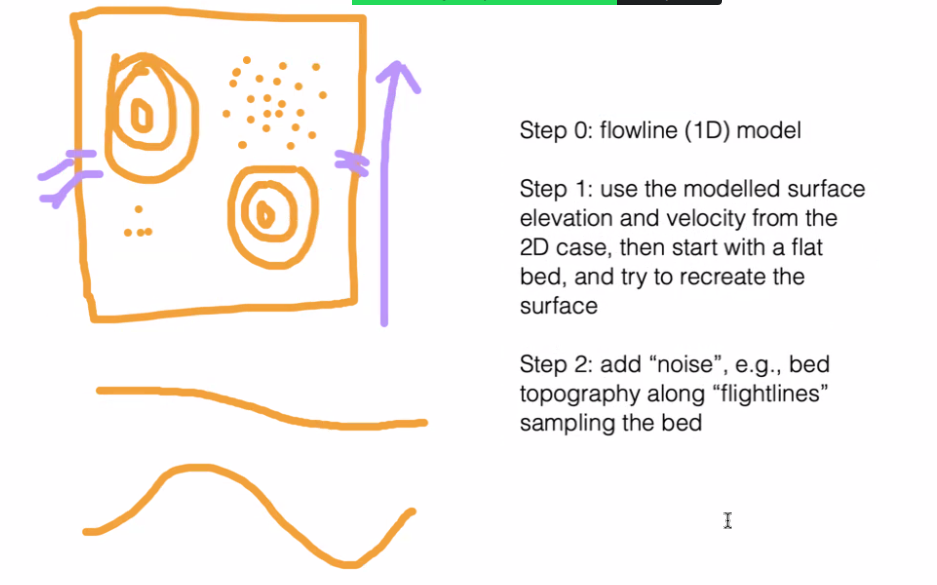
\includegraphics[width=0.9\linewidth]{steps.png}
\captionof{figure}{TODO}
\label{fig:first_sims}
\end{Figure}

\begin{Figure}
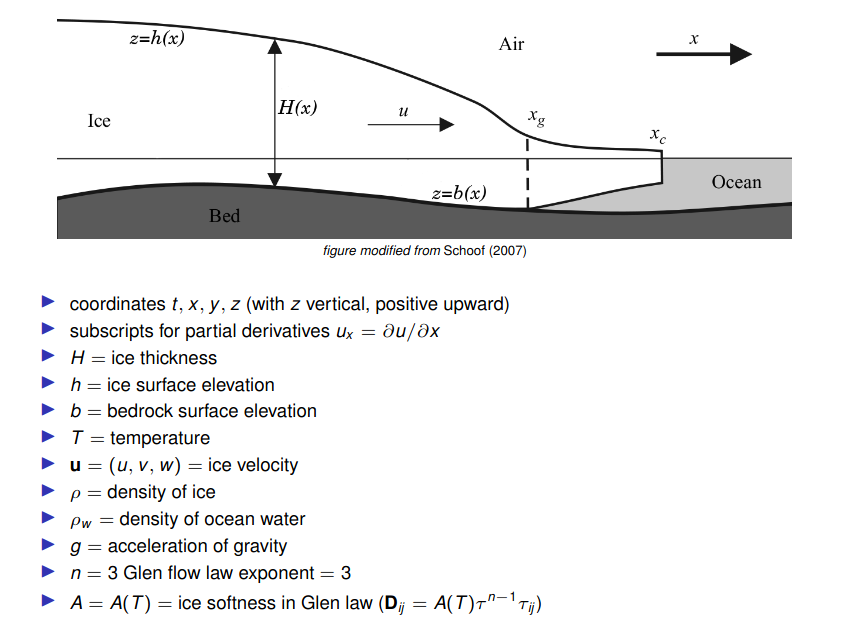
\includegraphics[width=0.9\linewidth]{numerical_modelling_of_glaciers.png}
\captionof{figure}{figure taken from\cite{modelling_ppt}}
\label{fig:parameters}
\end{Figure}

\section{ISSM: Continental-Scale Ice Sheet Modelling}
The Ice Sheet System Model (ISSM) was developed and is used for simulating ice sheet flow at continental scales. ISSM, a finite element, thermomechanical model, incorporates high-order stresses and high spatial resolution capabilities\cite{ISSM}. The Larour et al. (2012) ISSM paper discusses the different ice flow models within the software, including the full-Stokes, Blatter-Pattyn, Shallow-Shelf, and Shallow Ice Approximations, highlighting their individual strengths and limitations. It also explores numerical methods employed, such as static adaptive mesh refinement and inverse methods for parameter estimation. Finally, the study showcases the application of ISSM to the Greenland Ice Sheet, demonstrating its capacity to model the ice flow velocity with high accuracy, using data assimilation techniques to infer the basal drag coefficient.


% Study Guide
% Glossary of Key Terms

%     Shallow Ice Approximation (SIA): A simplified ice flow model that considers only vertical shear stresses and neglects horizontal stress gradients. Suitable for slow-moving ice in the interior of ice sheets.
%     Shallow Shelf Approximation (SSA): A simplified ice flow model that neglects vertical shear stresses and assumes depth-independent horizontal velocity. Appropriate for modeling floating ice shelves and fast-flowing ice streams.
%     Blatter-Pattyn Approximation (BP): A higher-order ice flow model that incorporates longitudinal stresses, making it suitable for simulating fast-flowing ice streams and regions with significant vertical shear.
%     Full-Stokes (FS): The most comprehensive and computationally expensive ice flow model, accounting for all stress components. Essential for accurately simulating ice flow near grounding lines.
%     Ice Sheet System Model (ISSM): A finite element, thermomechanical ice flow model that incorporates SIA, SSA, BP, and FS formulations to simulate ice sheet behaviour at various complexities and spatial resolutions.
%     Finite Element Method (FEM): A numerical method for solving partial differential equations by dividing the domain into smaller elements and approximating the solution within each element.
%     Adaptive Mesh Refinement: A technique used to refine the mesh in regions of high variability or complexity, enhancing model accuracy and efficiency.
%     Data Assimilation: The process of incorporating observational data into a model to improve its accuracy and predictive capabilities.
%     Basal Drag Coefficient: A parameter representing the frictional resistance between the ice sheet base and the underlying bedrock.
%     Grounding Line: The boundary where the ice sheet transitions from grounded ice to floating ice (ice shelf).
%     Calving: The process by which icebergs break off from the edge of a glacier or ice sheet.
%     InSAR: Interferometric Synthetic Aperture Radar, a remote sensing technique used to measure ice surface velocity.

% Quiz

% Instructions: Answer the following questions in 2-3 sentences.

%     What are the limitations of the Shallow Ice Approximation (SIA) and Shallow Shelf Approximation (SSA) in ice sheet modelling?
%     Why is the Full-Stokes (FS) model considered the most accurate representation of ice flow, and what makes its application challenging?
%     How does the Ice Sheet System Model (ISSM) integrate different ice flow approximations?
%     What is the importance of anisotropic adaptive mesh refinement in ISSM?
%     Describe the role of data assimilation in improving the accuracy of ice sheet models.
%     Why is the basal drag coefficient a crucial parameter in ice flow modeling?
%     Explain the concept of grounding line dynamics and its significance.
%     What is the process of calving, and why is it relevant to ice sheet mass balance?
%     How does ISSM handle the thermal regime of ice sheets?
%     What are some key challenges and future directions in ice sheet modeling using ISSM?

% Quiz Answer Key

%     SIA neglects horizontal stress gradients and is unsuitable for fast flow, while SSA ignores vertical shear, limiting accuracy near grounding lines.
%     FS accounts for all stress components, making it highly accurate, but its computational expense poses a challenge for large-scale applications.
%     ISSM offers SIA, SSA, BP, and FS formulations, allowing for different levels of complexity and computational efficiency.
%     It concentrates elements in dynamic regions like fast-flowing outlets, optimizing computational resources while preserving accuracy.
%     Data assimilation incorporates observations (e.g., surface velocity) to constrain model parameters and improve realism.
%     It governs basal friction, a key factor influencing ice flow velocity and the response to changes in temperature or basal conditions.
%     Grounding line dynamics refer to the movement of the grounding line, impacting ice discharge and contributing to sea level rise.
%     Calving is the breaking off of icebergs, a major process of mass loss from ice sheets, influencing their size and contribution to sea level.
%     ISSM includes a thermal model with heat conduction, advection, and a penalty scheme to ensure the temperature stays below the pressure melting point.
%     Challenges include improving grounding line dynamics, incorporating calving laws, and increasing spatial resolution, requiring more efficient numerical techniques and computational power.

% Essay Questions

%     Compare and contrast the four ice flow approximations (SIA, SSA, BP, and FS) implemented in ISSM, discussing their strengths, limitations, and appropriate applications.
%     Explain the process of data assimilation in ISSM, focusing on the inversion for the basal drag coefficient. Discuss the challenges and benefits of this approach.
%     Discuss the importance of accurate representation of grounding line dynamics in ice sheet models. What are the limitations of the current implementation in ISSM, and how can they be addressed in future development?
%     Describe the role of calving in ice sheet mass balance, and discuss the need to incorporate realistic calving laws in ice sheet models like ISSM.
%     Evaluate the potential of ISSM as a tool for projecting ice sheet contribution to future sea level rise. What are the key uncertainties and areas where the model can be improved?